\section {Implementation and Technical Notes}

Python 3.6 was used to code, with modularity of components being the main focus. \\

The code has been split into logical modules: \\
\begin{itemize}
\item \textbf{model\_lib.py}: defines the MNIST model. 
\item \textbf{mnist\_eager.py}: trains the MNIST model with \textit{tf eager execution}. 
\item  \textbf{README.md }: Contains relevant code documentation.
\end{itemize}


\section {Question 1}

We use \textit{tensorflow eager} to train the MNIST CNN Model of the following architecture:

\begin{lstlisting}
_________________________________________________________________
Layer (type)                 Output Shape              Param #   
=================================================================
reshape (Reshape)            (None, 1, 28, 28)         0         
_________________________________________________________________
conv2d (Conv2D)              (None, 32, 28, 28)        320       
_________________________________________________________________
max_pooling2d (MaxPooling2D) multiple                  0         
_________________________________________________________________
conv2d_1 (Conv2D)            (None, 32, 14, 14)        9248      
_________________________________________________________________
flatten (Flatten)            (None, 1568)              0         
_________________________________________________________________
dense (Dense)                (None, 500)               784500    
_________________________________________________________________
dropout (Dropout)            (None, 500)               0         
_________________________________________________________________
dense_1 (Dense)              (None, 10)                5010      
=================================================================
Total params: 799,078
Trainable params: 799,078
Non-trainable params: 0
_________________________________________________________________
\end{lstlisting}

The code to train the model is:

\begin{lstlisting}
python3 mnist/mnist_eager.py
\end{lstlisting}

\begin{itemize}
\item Learning rate of $1e-4$, with SGD momentum was used as the optimiser.
\item We periodically run evaluation post an epoch. The files are recorded as tensorboard events.
\item Logs are stored at \textit{/tmp/tensorflow/mnist}, with seperate directories for \textit{train},\textit{eval},\textit{occlusion},\textit{filters},\textit{activations} and \textit{adversarial attacks}.
\end{itemize}


We use tensorboard for logs, which can be viewed by:
\begin{lstlisting}
tensorboard --log_dir /tmp/tensorflow/mnist
\end{lstlisting}

We report a test accuracy of $99.11$, and with the cross entropy loss well below $0.03$.

\subsection{Accuracy and Loss curves}

\begin{figure}[ht]
\centering
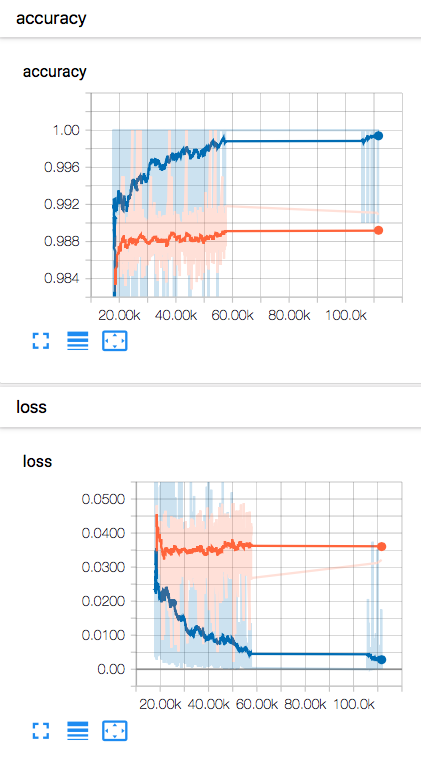
\includegraphics[angle=0,width=0.75\textwidth]{assign-2/logs/train/TensorBoard.png}
\caption{Accuracy Loss curves for \textbf{MNIST CNN}}
\end{figure}

\subsection{Accuracy and Loss curves (with batch norm)}

We note slightly faster convergence with batch normalisation.

\begin{figure}[ht]
\centering
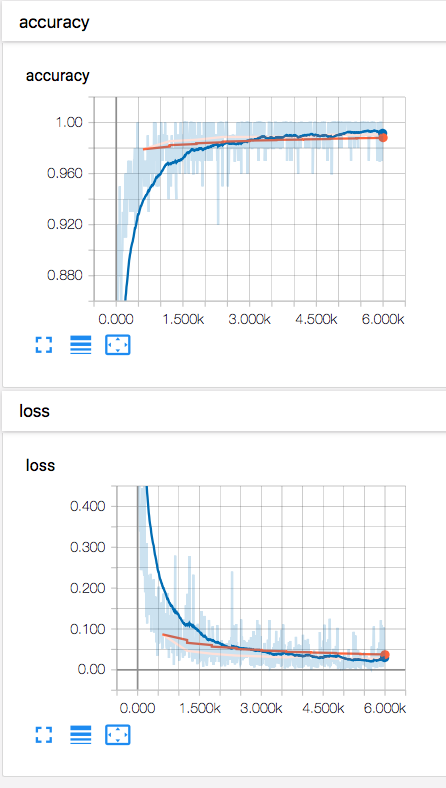
\includegraphics[angle=0,width=0.8\textwidth]{assign-2/logs/train/bn.png}
\caption{Accuracy Loss curves with batch-norm for \textbf{MNIST CNN}}
\end{figure}


\subsection {Code Blocks (model definition)}
\begin{lstlisting}
def create_model(data_format='channels_first'):
    """Model to recognize digits in the MNIST dataset.

    Args:
    * data_format: NHWC or NCHW. Prefer latter for CPUs, former for GPUs.

    Returns:
      A tf.keras.Model.
    """
    if data_format == 'channels_first':
        input_shape = [1, 28, 28]
    else:
        assert data_format == 'channels_last'
        input_shape = [28, 28, 1]

    l = tf.keras.layers
    max_pool = l.MaxPooling2D(
        (2, 2), (2, 2), padding='same', data_format=data_format)
    # The model consists of a sequential chain of layers, so tf.keras.Sequential
    # (a subclass of tf.keras.Model) makes for a compact description.
    return tf.keras.Sequential(
        [
            l.Reshape(
                target_shape=input_shape,
                input_shape=(28 * 28,)),
            l.Conv2D(
                32,
                3,
                padding='same',
                data_format=data_format,
                activation=tf.nn.relu),
            max_pool,
            l.Conv2D(
                32,
                3,
                padding='same',
                data_format=data_format,
                activation=tf.nn.relu),
            max_pool,
            l.Flatten(),
            l.Dense(500, activation=tf.nn.relu),
            l.Dropout(0.4),
            l.Dense(10)
        ])
\end{lstlisting}

We run the list of properties for all possible GPU's present in the given machine.

\bigskip

\subsection{Sample Outputs}

\begin{figure}[h]
\begin{subfigure}
\centering

\includegraphics[angle=0,width=0.4\textwidth]{assign-2/logs/0.png}
\caption{Sample Output: label 0, prediction 0, probability 0.992}
\end{subfigure}
\begin{subfigure}
\centering
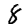
\includegraphics[angle=0,width=0.4\textwidth]{assign-2/logs/8.png}
\caption{Sample Output: label 8, prediction 8, probability 0.873}
\end{subfigure}
\end{figure}

\section{Question 2}

Visualising Filters and Activations:

(We skip some of the visualisations for brevity)

\subsection{Filters (first conv layer)}
\begin{figure}[!htbp]
\begin{subfigure}
\centering
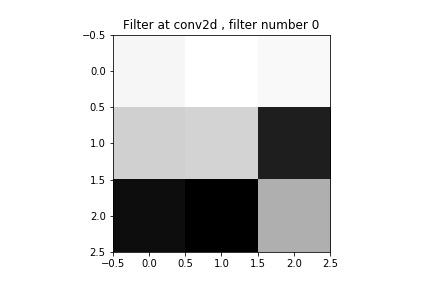
\includegraphics[angle=0,width=0.4\textwidth]{assign-2/logs/vis/filter-conv2d-0.jpg}
\caption{Filter-0}
\end{subfigure}
\begin{subfigure}
\centering
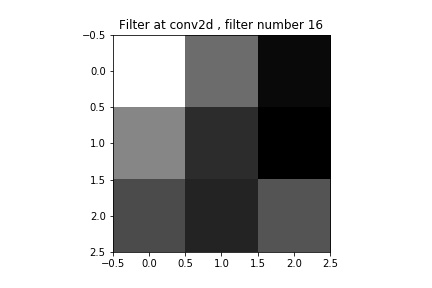
\includegraphics[angle=0,width=0.4\textwidth]{assign-2/logs/vis/filter-conv2d-16.jpg}
\caption{Filter-16}
\end{subfigure}
\begin{subfigure}
\centering
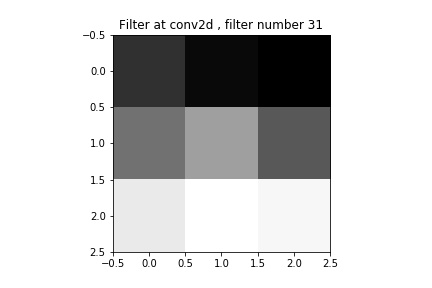
\includegraphics[angle=0,width=0.4\textwidth]{assign-2/logs/vis/filter-conv2d-31.jpg}
\caption{Filter-31}
\end{subfigure}
\end{figure}

\subsection{Filters (second conv layer)}

\begin{figure}[!htbp]
\begin{subfigure}
\centering
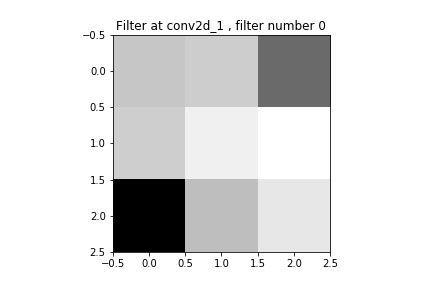
\includegraphics[angle=0,width=0.4\textwidth]{assign-2/logs/vis/filter-conv2d_1-0.jpg}
\caption{Filter-0}
\end{subfigure}
\begin{subfigure}
\centering
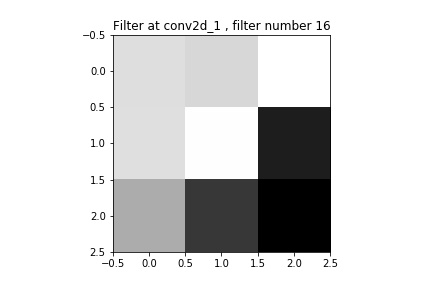
\includegraphics[angle=0,width=0.4\textwidth]{assign-2/logs/vis/filter-conv2d_1-16.jpg}
\caption{Filter-16}
\end{subfigure}
\begin{subfigure}
\centering
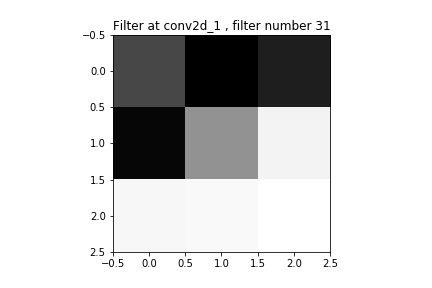
\includegraphics[angle=0,width=0.4\textwidth]{assign-2/logs/vis/filter-conv2d_1-31.jpg}
\caption{Filter-31}
\end{subfigure}
\end{figure}

\subsection{Activations (first conv layer)}

\begin{figure}[!htbp]
\begin{subfigure}
\centering
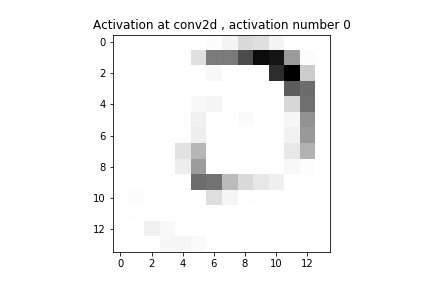
\includegraphics[angle=0,width=0.4\textwidth]{assign-2/logs/vis/activation-conv2d-0.jpg}
\caption{Activation-0}
\end{subfigure}
\begin{subfigure}
\centering
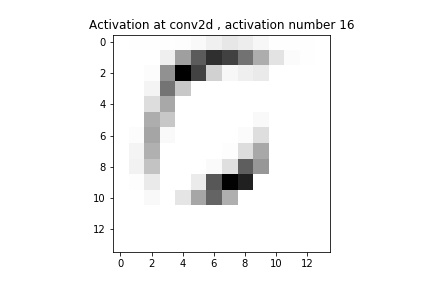
\includegraphics[angle=0,width=0.4\textwidth]{assign-2/logs/vis/activation-conv2d-16.jpg}
\caption{Activation-16}
\end{subfigure}
\begin{subfigure}
\centering
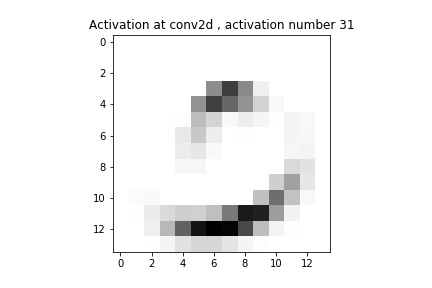
\includegraphics[angle=0,width=0.4\textwidth]{assign-2/logs/vis/activation-conv2d-31.jpg}
\caption{Activation-31}
\end{subfigure}
\end{figure}

\subsection{Activations (second conv layer)}

\begin{figure}[!htbp]
\begin{subfigure}
\centering
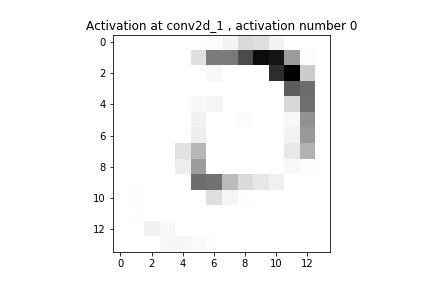
\includegraphics[angle=0,width=0.4\textwidth]{assign-2/logs/vis/activation-conv2d_1-0.jpg}
\caption{Activation-0}
\end{subfigure}
\begin{subfigure}
\centering
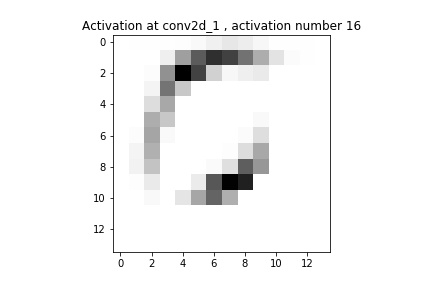
\includegraphics[angle=0,width=0.4\textwidth]{assign-2/logs/vis/activation-conv2d_1-16.jpg}
\caption{Activation-16}
\end{subfigure}
\begin{subfigure}
\centering
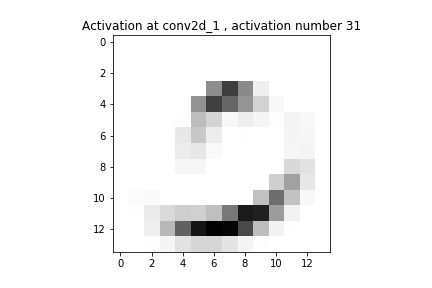
\includegraphics[angle=0,width=0.4\textwidth]{assign-2/logs/vis/activation-conv2d_1-31.jpg}
\caption{Activation-31} 
\end{subfigure}
\end{figure}

\subsection{Occlusion Probabilities}

We perform occlusion variation as a function of pixel distance by using a white patch to block the area. The patch size is $6*6$. \\

\begin{figure}[!htbp]
\begin{subfigure}
\centering
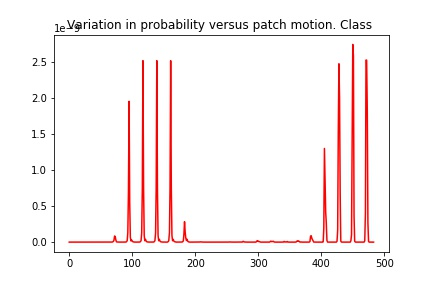
\includegraphics[angle=0,width=0.7\textwidth]{assign-2/logs/occ/1d-var-7.jpg}
\caption{1D Probability variation for occlusion of 7.}
\end{subfigure}
\begin{subfigure}
\centering
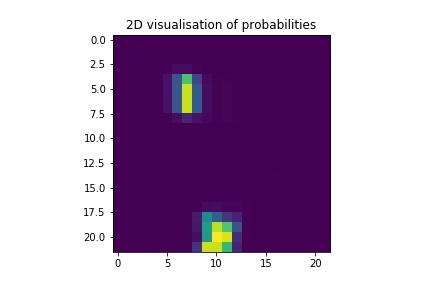
\includegraphics[angle=0,width=0.7\textwidth]{assign-2/logs/occ/2d-var-7.jpg}
\caption{2D Probability variation (heatmap) for occlusion of 7.}
\end{subfigure}
\end{figure}

\section{Question 3 }

We now work on different adversarial attacks, targeted, non-targeted, adding noise. 

\subsection{Non-Targeted}

We define the adversarial cost for gradient ascent as:

$$ C = loss(\vec y_{goal}, y_{hat}(\vec x))+ \lambda \|\vec x |^2_2 $$

Here, the loss used was cross entropy with the swapped labels. Regularisation with respect to the inputs was done as an optional exercise, and we noted improvements in the adversarial attack image quality. These are reported in figures 18 to 20.

\begin{figure}[!htbp]
\begin{subfigure}
\centering
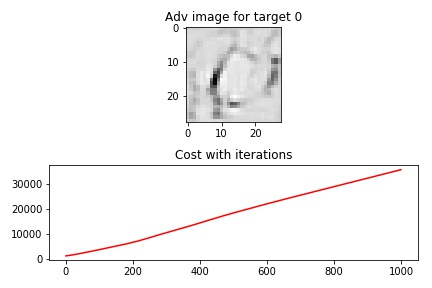
\includegraphics[angle=0,width=0.65\textwidth]{assign-2/logs/adv/non/adv-0.jpg}
\caption{Digit 0, Non targeted attack}
\end{subfigure}
\begin{subfigure}
\centering
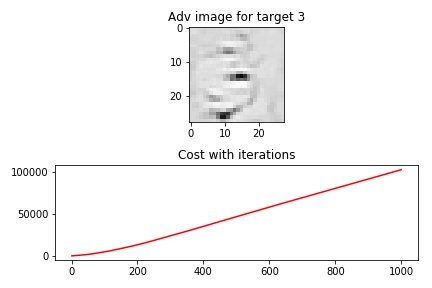
\includegraphics[angle=0,width=0.65\textwidth]{assign-2/logs/adv/non/adv-3.jpg}
\caption{Digit 3, Non targeted attack}
\end{subfigure}
\begin{subfigure}
\centering
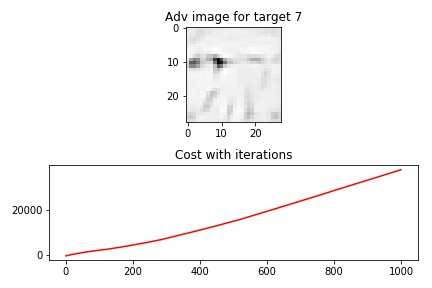
\includegraphics[angle=0,width=0.65\textwidth]{assign-2/logs/adv/non/adv-7.jpg}
\caption{Digit 7, Non targeted attack} 
\end{subfigure}
\end{figure}

\subsection{Targeted}
The cost function in this case becomes:
$$ C = \|\vec y_{goal} - y_{hat}(\vec x)\|^2_2 + \lambda \|\vec x - \vec x_{target}\|^2_2 $$

We try out a variant with cross-entropy instead of MSE for comparing labels, which turns out to me more optimal. These are reported in figures 21 to 23. For brevity, we have not included the cost variation, which is more or less similar.



\begin{figure}[!htbp]
\begin{subfigure}
\centering
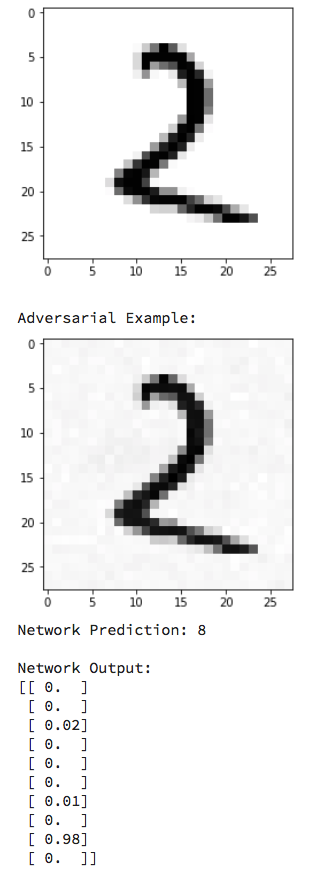
\includegraphics[angle=0,width=0.5\textwidth]{assign-2/logs/adv/tar/2.png}
\caption{Digit 2, targeted to be 8 }
\end{subfigure}
\end{figure}
\begin{figure}[!htbp]
\begin{subfigure}
\centering
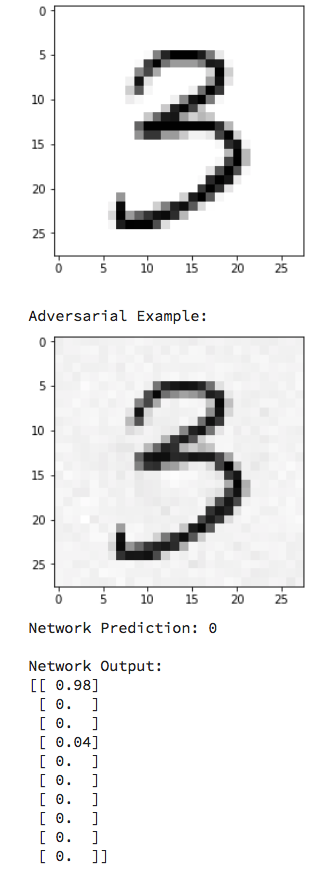
\includegraphics[angle=0,width=0.5\textwidth]{assign-2/logs/adv/tar/3.png}
\caption{Digit 3, targeted to be 0.}
\end{subfigure}
\end{figure}

\subsection{Adding Noise }

Here, 
$$ C = \|\vec y_{goal} - y_{hat}(\vec x)\|^2_2  $

But with the noise composing the image as;

$$x_{noise}=x + noise$$

\section{Question 3}

We use a LSTM for this question with hidden (state) size as 5. We notice that increasing this to 10 improves accuracy (nearly 100\%) and decreasing to 2 lowers accuracy. These plots however, aren't included here, and we experiment with state size 5.

Hyper-parameters:
\begin{itemize}
\item  Adam optimiser, lr = 0.01, beta1 = 0.9, beta2 = 0.99
\item  Loss : MSE and Cross Entropy
\item  Single hidden layer, 5 units wide.
\end{itemize}

\subsection{MSE vs Cross Entropy}
We also note that MSE performs much better than Cross Entropy. This is because the output sequence is a binary number and their probabilities are correlated. Hence, we cannot use a "clean" version of cross entropy with $L$ distinct distributions. We use a hackish method to use cross entropy, and for the reasons noted above, it performs poorly.

\begin{figure}[!htbp]
\begin{subfigure}
\centering
\includegraphics[angle=0,width=0.65\textwidth]{assign-3/logs/}
\caption{$L=5$, Cross Entropy Loss}
\end{subfigure}
\begin{subfigure}
\centering
\includegraphics[angle=0,width=0.65\textwidth]{assign-3/logs/}
\caption{$L=5$, MSE Loss}
\end{subfigure}
\end{figure}



 